\documentclass{article}

\usepackage{fancyhdr}
\usepackage{extramarks}
\usepackage{amsmath}
\usepackage{amsthm}
\usepackage{amsfonts}
\usepackage{tikz}
\usepackage[plain]{algorithm}
\usepackage{algpseudocode}

\usetikzlibrary{automata,positioning}

%
% Basic Document Settings
%

\topmargin=-0.45in
\evensidemargin=0in
\oddsidemargin=0in
\textwidth=6.5in
\textheight=9.0in
\headsep=0.25in

\linespread{1.1}

\pagestyle{fancy}
\lhead{\hmwkAuthorName}
\chead{\hmwkClass\ (\hmwkClassInstructor\ \hmwkClassTime): \hmwkTitle}
\rhead{\firstxmark}
\lfoot{\lastxmark}
\cfoot{\thepage}

\renewcommand\headrulewidth{0.4pt}
\renewcommand\footrulewidth{0.4pt}

\setlength\parindent{0pt}

%
% Create Problem Sections
%

\newcommand{\enterProblemHeader}[1]{
    \nobreak\extramarks{}{Problem \arabic{#1} continued on next page\ldots}\nobreak{}
    \nobreak\extramarks{Problem \arabic{#1} (continued)}{Problem \arabic{#1} continued on next page\ldots}\nobreak{}
}

\newcommand{\exitProblemHeader}[1]{
    \nobreak\extramarks{Problem \arabic{#1} (continued)}{Problem \arabic{#1} continued on next page\ldots}\nobreak{}
    \stepcounter{#1}
    \nobreak\extramarks{Problem \arabic{#1}}{}\nobreak{}
}

\setcounter{secnumdepth}{0}
\newcounter{partCounter}
\newcounter{homeworkProblemCounter}
\setcounter{homeworkProblemCounter}{1}
\nobreak\extramarks{Problem \arabic{homeworkProblemCounter}}{}\nobreak{}

\newenvironment{homeworkProblem}{
    \section{Problem \arabic{homeworkProblemCounter}}
    \setcounter{partCounter}{1}
    \enterProblemHeader{homeworkProblemCounter}
}{
    \exitProblemHeader{homeworkProblemCounter}
}

%
% Homework Details
%   - Title
%   - Due date
%   - Class
%   - Section/Time
%   - Instructor
%   - Author
%

\newcommand{\hmwkTitle}{Homework\ \#3}
\newcommand{\hmwkDueDate}{June 7, 2019}
\newcommand{\hmwkClass}{Introduction to Cryptography}
\newcommand{\hmwkClassTime}{}
\newcommand{\hmwkClassInstructor}{Professor Manuel}
\newcommand{\hmwkAuthorName}{ShiHan Chan}

%
% Title Page
%

\title{
    \vspace{2in}
    \textmd{\textbf{\hmwkClass:\ \hmwkTitle}}\\
    \normalsize\vspace{0.1in}\small{Due\ on\ \hmwkDueDate\ at 3:10pm}\\
    \vspace{0.1in}\large{\textit{\hmwkClassInstructor\ \hmwkClassTime}}
    \vspace{3in}
}

\author{\textbf{\hmwkAuthorName}}
\date{}

\renewcommand{\part}[1]{\textbf{\large Part \Alph{partCounter}}\stepcounter{partCounter}\\}

%
% Various Helper Commands
%

% Useful for algorithms
\newcommand{\alg}[1]{\textsc{\bfseries \footnotesize #1}}

% For derivatives
\newcommand{\deriv}[1]{\frac{\mathrm{d}}{\mathrm{d}x} (#1)}

% For partial derivatives
\newcommand{\pderiv}[2]{\frac{\partial}{\partial #1} (#2)}

% Integral dx
\newcommand{\dx}{\mathrm{d}x}

% Alias for the Solution section header
\newcommand{\solution}{\textbf{\large Solution}}

% Probability commands: Expectation, Variance, Covariance, Bias
\newcommand{\E}{\mathrm{E}}
\newcommand{\Var}{\mathrm{Var}}
\newcommand{\Cov}{\mathrm{Cov}}
\newcommand{\Bias}{\mathrm{Bias}}

\begin{document}

\maketitle

\pagebreak

\begin{homeworkProblem}

    \textbf{Part One}\\
	Possible factors of $X^2+1$ in $F_3[X]$ are X,X+1,X+2, try combination one by one:\\
	$X*X=X^2\neq X^2+1$\\
	$X(X+1)=X^2+X\neq X^2+1$\\
	$X(X+2)=X^2+2X\neq X^2+1$\\
	$(X+1)(X+1)=X^2+2X+1\neq X^2+1$\\
	$(X+1)(X+2)=X^2+3X+2=X^2+2\neq X^2+1$\\
	$(X+2)(X+2)=X^2+4X+4=X^2+X+1\neq X^2+1$\\
	So $X^2+1$ is irreducible in $F_3[X]$.
	
	\textbf{Part Two}\\
	According to theorem on lecture slide: if P(X) is irreducible and A(X) is a polynomial in finite field, then there exists a polynomial B(x) such that $A(X)B(X)\equiv 1 \mod P(X)$\\
	Let $P(X)=X^2+1, A(X)=1+2X$, B(X) is the multiplicative inverse of $1+2X \mod X^2+1$\\
    
    \textbf{Part Three}\\
    Use extended euclidean algorithm to find B(X): (All calculations are in $F_3[X]$)\\ 
    $(1+2X)B(X)-1=(X^2+1)*N(X)$\\
    $(X^2+1)=(2X+1)*(2X+2)+2$\\
    multiply both sides by 2 we can get:\\
    $2(X^2+1)=(2X+1)*(X+1)+1$\\
    $(1+2X)*(2X+2)-1=(X^2+1)$\\
    $B(X)=2x+2$
\end{homeworkProblem}

\pagebreak


\begin{homeworkProblem}
1. (a)\\
"InvShiftrows" operation cyclically shift to the right row i by offset i, $0 \le i \le 3$\\
(b)\\
If we xor a value by another same value twice, it would generate the same value. So the inverse of AddRoundKey is same as AddRoundKey. XOR the ciphertext and key will generate the plaintext.\\
ex. $a \oplus b = c \equiv c \oplus b = a$\\
(c)\\
Since if we multiply matrix B in InvMixColumn with matrix A in MixColumn, we would have an identity matrix I.
Note that when we multiply elemnts in two matrix, we must multiply elements in corresponding position and use xor operation to add them together.\\
ex. For element in third row and third column, $(00001101 * 00000001)\oplus (00001001*00000011) \oplus (00001110 * 00000010)\oplus (00001011 * 00000001) = 00000001$\\
After calculation for each element, we get BA=I\\
In other words, suppose original matrix is O, then B(AO)=(BA)O=IO=O\\
2.\\
(1). Generate round keys by the key, then we apply AddroundKey operation.\\
(2). We apply 9 rounds of four operations in order: InvShiftRow, InvShiftByte, AddRoundKey and InvMixColumn.\\
(3). We apply InvShiftRow, InvSubbyte and AddRoundKey operation.\\

3.\\
 Since InvSubByte operation only replace value of a cell by original value of the cell, and InvShiftRow operation doesn't change value of any cell, so the order will not influence the result. That explains why they can be applied in reverse order.\\
 4. (a)\\
 Since both operations use external things (matrix, key) to affect the output value, the reverse order may generate a different result.\\
 (b)\\
 $[(m_{i,j})(a_{i,j})]\oplus k_{i,j}$\\
 (c)\\
 $e_{i,j}=[(m_{i,j})(a_{i,j})]\oplus (k_{i,j}) \implies (a_{i,j})=(m_{i,j})^{-1}((e_{i,j})\oplus (k_{i,j}))=(m_{i,j})^{-1}(e_{i,j})\oplus (m_{i,j})^{-1}(k_{i,j})$\\
 So the inverse operation is:\\
 $(e_{i,j}) \rightarrow (m_{i,j})^{-1}(e_{i,j})\oplus (m_{i,j})^{-1}(k_{i,j})$\\
 (d)\\
 We can transform the InvAddRoundKey $k'$ operation to first apply InvMixColumn operation $m^{-1}$ to the key, then apply AddRoundKey  operation.\\
 ex. $m^{-1}(a\oplus k)=m^{-1} a\oplus m^{-1} k =m^{-1} a \oplus k'$

 
 5.\\
 (1). Generate round keys by the key, then we apply AddroundKey operation.\\
 (2). We apply 9 rounds of four operations in order: InvShiftRow, InvShiftByte, AddRoundKey and InvMixColumn.\\
 (3). We apply InvShiftRow, InvSubbyte and AddRoundKey operation.\\
 
 6.\\
 We just need to implement four inverse transformation to decrypt the message. So if we know the encrypt method, we can easily derive the decrypt method.\\
 
 
 
  


\end{homeworkProblem}
\pagebreak
\begin{homeworkProblem}
1.\\
The length of plaintext in DES is 64 bits \\
(a)The order of plaintext's element is transformed by following table:\\
\begin{figure}[h]
	\graphicspath{images}
	\begin{center}
		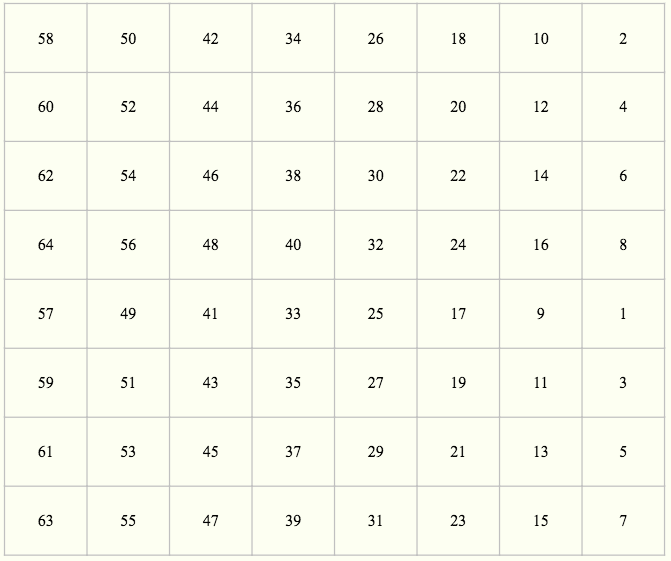
\includegraphics[scale=0.3,command=Figure1: IP]{images/1.png}
	\end{center}
\end{figure} 
\\
For example, the new 2th bit is old 50th bit.\\
After transformation, the plaintext is divided to two part of 32 bits. And we apply Feistel Network for 16 rounds, each turn can be shown by following picture:\\
\begin{figure}[h]
	\graphicspath{images}
	\begin{center}
		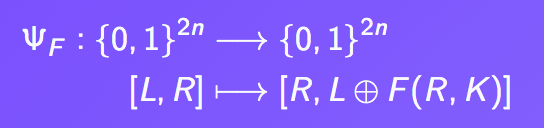
\includegraphics[scale=0.3,command=Figure1: IP]{images/2.png}
	\end{center}
\end{figure} 
\\
The function F(R,K) works in the following procedure procedure: expansion, key mixing, substitution, permutation.\\
After 16 rounds of Feistel Network, we transform the output of the network by following table and get the ciphertext.\\
\begin{figure}[h]
	\graphicspath{images}
	\begin{center}
		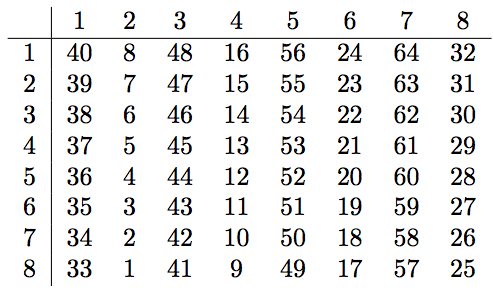
\includegraphics[scale=0.3,command=Figure1: IP]{images/3.png}
	\end{center}
\end{figure} 
\\
For decryption of DES, we just reverse the transformation table and reverse the order of key table K.\\
2.\\
In linear cryptanalysis, we try to use linear approximation to build the relationship between plaintext, key and ciphertext. For example, if ciphertext=f(plaintext, key), we try to find linear approximation of f. After getting the linear approximation of the non-linear part, we combine it with other linear part. Then, we use the linear equation with plaintext-ciphertext pair to enumerate possible private keys.\\
In differential cryptaanalysis, this attack aims to obeserve plaintext/ciphertext difference pattern. For some pieces of input plaintext, try to observe how the difference of plaintext affects the difference of ciphertext, and use this difference to guess the possible key value.\\ 
3.\\
Since people can use meet in the middle attack on double DES, the safety of double DES is similar to single DES.\\
Suppose plaintext is P, ciphertext is C, K1, K2 are two keys, f1 is encrypt function, f2 is decrypt function of double DES.\\ 
$C=f_{1}(f_1(P,K1),K2)$\\
$P=f_{2}(f_2(C,K2),K1)$\\
If we have a pair of plaintext-ciphertext pair, we can enumerate all possible key K1 and store all the middle result I. It takes $2^{56}$ operation to enumerate all key, calculate the middel result $I=f_{1}(P,K1)$ and some space to store the middle result. Then we enumerate all possible key K2 and calculate the middle result $I=f_{2}(C,K2)$, for each middle result, check whether there is a same result in space. If we find one, K1,K2 are correct keys with high probability. We only need $2^{57}$ operation and some space since we can check whether there is a same result in O(1) time (hash table).\\
For triple DES,\\
$C=f_{1}(f_{2}(f_1(P,K1),K2),K3)$\\
$P=f_{2}(f_{1}(f_2(C,K3),K2),K1)$\\
If K1=K2=K3, it is same as single DES, and it provides compatibility. If K1,K2 are independent, K1=K3,  although it only has two keys, it is safer than double DES since if people apply meet in the middle attack, it takes $2^{112}$ operations to enumerate the middle result and find the private key. If K1,K2,K3 are all independent, meet in the middle attack still takes $2^{112}$ operations to find the private key.\\
Since triple DES has compatibility and it's safer, it is used more often than double DES nowadays.\\

4.\\
If we type "man passwd" in cmd, we might spot that UNIX encryption method is single DES and user's password is stored in /etc/passwd file. But single DES is not safe nowadays. New Unix version uses more security method to encrypt password such as SHA.

\end{homeworkProblem}
\begin{homeworkProblem}
Programming Part
\end{homeworkProblem}
\end{document}
